\subsection{VQ-GAN – Vector Quantized Generative Adversarial Network}
\begin{frame}[allowframebreaks]{VQ-GAN}
    \large VQ-GAN – Vector Quantized Generative Adversarial Network \\[1em]
    \textbf{VQ-GAN} is a generative model that combines the strengths of vector quantization and GANs to generate high-quality images.

    \begin{itemize}
        \item \textbf{Vector Quantization:} Encodes images into discrete latent codes, allowing for efficient representation and generation.
        \item \textbf{GAN Framework:} Uses a discriminator to guide the generator in producing realistic images.
        \item \textbf{Applications:} Image synthesis, super-resolution, and style transfer.
    \end{itemize}
\framebreak
    \textbf{Architecture:} VQ-GAN consists of an encoder, a quantizer, a decoder, and a discriminator.
    \begin{itemize}
        \item \textbf{Encoder:} Maps input images to a continuous latent space.
        \item \textbf{Quantizer:} Discretizes the continuous latent space into a finite set of codes.
        \item \textbf{Decoder:} Reconstructs images from the quantized latent codes.
        \item \textbf{Discriminator:} Evaluates the realism of generated images, providing feedback to the generator.
    \end{itemize}
\framebreak
    \begin{figure}
        \centering
        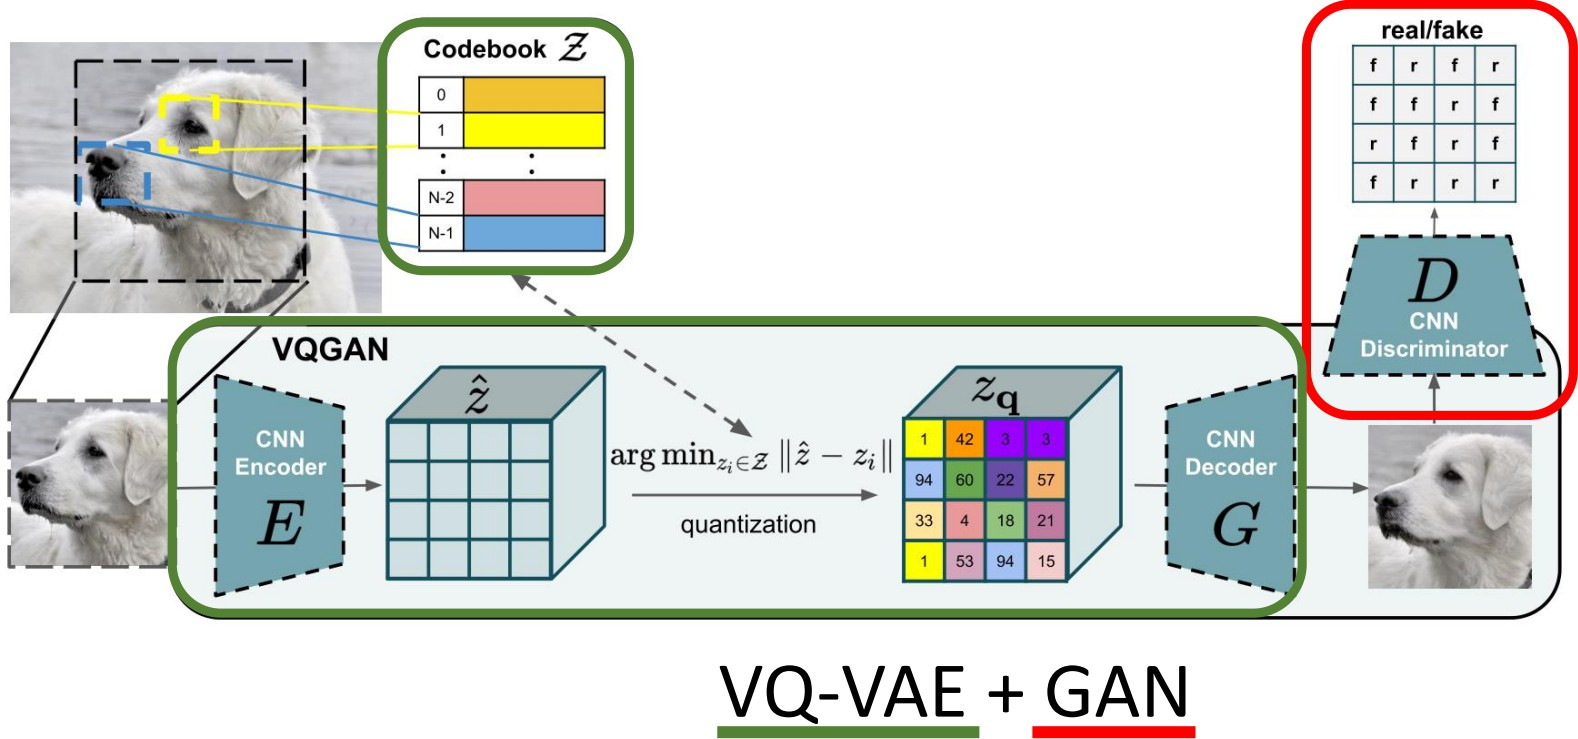
\includegraphics[width=1\textwidth,height=0.9\textheight,keepaspectratio]{images/video/slide_59_1_img.jpg}
    \end{figure}
\end{frame}
